\chapter{Introduzione}

\section{Obiettivo di progetto} 
La presente tesi è stata sviluppata a partire da una task affidatami durante la mia esperienza di tirocinio presso l'azienda REA Robotics nel periodo compreso tra il 2 settembre 2024 e l'11 ottobre 2024. Nello specifico, il team mi ha chiesto di creare una piattaforma SCADA per impianti custom che potesse rispettare linee guida moderne, attraverso l'utilizzo di un nuovo software di sviluppo e gestione. La principale necessità dell'azienda era di favorire l'integrazione tra più impianti di diversa tipologia per poter creare un ecosistema modulare, che funzionasse su tutte le macchine, indipendentemente da:
\begin{itemize}
    \item Tipologia di impianto
    \item Hardware utilizzato
    \item Sistema operativo installato
    \item Modalità d'uso del sistema
\end{itemize}
Questo approccio mirava a standardizzare le interazioni tra i diversi impianti, semplificando gestione e migliorando l'efficienza per gli aggiornamenti. Sin da subito il tirocinio era incentrato sull'affiancamento al team di sviluppo software di REA, per poter conoscere le metodologie di sviluppo interconnesso tra ingegneri SCADA e tecnici PLC, con l'obiettivo di imparare a collaborare in modo efficiente in team ed acquisire una prospettiva concreta del contesto lavorativo. Inoltre, un altro obiettivo era di ampliare le competenze tecniche nel campo dell'automazione industriale, con particolare attenzione alla progettazione di sistemi SCADA. Grazie al progetto, ho avuto l'opportunità di approfondire l'uso di strumenti specifici, come il software FactoryTalk Optix™, e di consolidare conoscenze già acquisite durante il percorso di studi, come la gestione di database e la progettazione di interfacce HMI. Un altro aspetto cruciale è stato sviluppare competenze trasversali, tra cui comunicazione efficace e risolvere problemi complessi adottando un approccio analitico in linea con le esigenze aziendali.

\section{L'azienda: REA Robotics Srl}

\begin{figure} [ht]
    \centering
    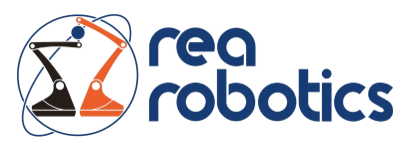
\includegraphics[width=0.5\linewidth]{Immagini/LogoREA.png}
    \caption{Logo REA Robotics. Fonte: \cite{rearoboticsLOGO}}
    \label{fig:LogoREA.png}
\end{figure}

Il gruppo REA opera da oltre 30 anni nel contesto industriale nazionale. Agli albori partner tecnologico dei primi costruttori di robot europei, nei primi anni si è focalizzata nel settore tradizionale della saldatura per poi estendere la propria esperienza nella General Industry: dall'automotive alle fonderie, fino ai giorni nostri includendo plastica e vetro. Oggi REA conta un organico in grado di coprire le principali aree di un'azienda moderna di automazione robotizzata, con particolare risalto alla Ricerca\&Sviluppo, all'avanprogettazione, oltre a disporre di tecnici con esperienza consolidata nell'ambito della manutenzione degli impianti e dell'assistenza post-vendita.\textsuperscript{\cite{spaziowebpdf}}

\subsection{La Mission}
\textit{Ci assumiamo la responsabilità di generare risultati garantendo a ogni cliente le soluzioni strategiche e i sistemi produttivi più efficienti, guidati dal nostro know-how trasversale nel mondo dell'industria. Sfruttando le nuove tecnologie in ottica 4.0, vogliamo diffondere l'automazione industriale attraverso sistemi integrati solidi e flessibili, disegnati a misura di ogni realtà.}\textsuperscript{\cite{rearobotics}}

\subsection{Settori e applicazioni}
La saldatura rappresenta per REA l'applicazione più storica e più conosciuta, essendo il settore in cui l'azienda sviluppa e anticipa le migliori soluzioni in termini di isole robotizzate da più di 30 anni. Le principali tecnologie usate dagli impianti robotizzati di saldatura sono: MIG–MAG (saldatura a filo), TIG con e senza metallo di apporto, plasma con e senza metallo di apporto, laser, saldobrasatura MIG, brasatura induzione, resistenza, riporti anti-usura MIG-MAG. Un'altra applicazione riguarda il taglio termico, campo in cui l'automazione può e potrà dare i maggiori benefici rispetto all'attuale esecuzione del taglio manuale. REA Robotics, nella sua pluriennale esperienza, realizza inoltre impianti di manipolazione per asservimento macchine e per assemblaggi industriali perfettamente adatte al processo produttivo del cliente e allo stesso tempo ridurre i costi, che è un imperativo imprescindibile. In collaborazione con una delle più importanti aziende costruttrici di impianti per il taglio e la lavorazione della lamiera, REA ha sviluppato un sistema robotizzato di asservimento a presse piegatrici. La novità, e la caratteristica principale di tale sistema, è di avere un sistema meccanico dotato di encoder applicabile a qualsiasi pressa che permette al robot di inseguire la pressa durante il suo movimento senza mai rilasciare la lamiera. Infine REA realizza celle robotizzate di pallettizzazione specificatamente studiate per inserimento nei fine linea dei processi produttivi, con soluzioni complete pensate per ogni specifico prodotto del cliente, dalla pallettizzazione di inscatolati, ruote fino alla pallettizzazione di profili d'acciaio.\textsuperscript{\cite{spaziowebpdf}}

\subsection{Robot utilizzati}
REA propone robot industriali di marchi come \textbf{ABB}, \textbf{Kuka} e \textbf{OTC Daihen} che comprendono le diverse applicazioni citate precedentemente.